\section{Semaine 19 : 12/06/2023 - 16/06/2023}
\graphicspath{{semaines/semaine_19/images/}}

\begin{abstract}
	\noindent
	\begin{enumerate}[label=\textbullet]
		\item Cette semaine, on a commencé par essayer de comprendre pourquoi le kernel se bloquait. On a tenté de résoudre un problème de correction sur une solution analytique avec nb\_vert=300 et en degré 10 et il n'y a pas eut de soucis. C'est pourquoi, je ne comprends pas pourquoi on a ce problème !
		\item Comme on ne peut pas faire du haut degré avec Legendre, j'ai testé avec des plus petits degrés. J'ai remarqué que la projection de phi\_tild sur notre espace de fonction V\_ex pour calculer la norme L2 d'erreur prend beaucoup de temps. Avec un degré 5, on est sur environ 15s (que l'on doit multiplier par nb\_data=100 et nb\_epochs=8). Par la suite, j'ai eut un autre problème avec la correction par multiplication. En prenant P=4 polynômes de Legendre, j'obtiens exactement les mêmes erreurs pour $\tilde{\phi}$ de degré 3 ou 5. En prenant P=6 et un degré 5, mes erreurs sont moins bonnes qu'avec P=4.
		\item J'ai alors testé la convergence de la décomposition en série de Polynômes de Legendre, tout d'abord avec la méthode des trapèzes pour différents nombres de points $N$. Puis avec une méthode de quadrature de scipy (\href{https://docs.scipy.org/doc/scipy/reference/generated/scipy.integrate.quad.html#scipy.integrate.quad}{scipy.integrate.quad}) qui prend une expression analytique de notre fonction en paramètre (et pas un ensemble de valeurs à des points connus). Il semblerait alors qu'avec la méthode de scipy, on est bien la convergence attendue.
		\item J'ai également corrigé la preuve sur l'inégalité pour le rehaussement avec FEM et ait commencé à générer une documentation sphinx du code.
	\end{enumerate}
\end{abstract}

\subsection{Test pour le kernel}

Test pour voir si le kernel se bloque sur la solution analytique en $\mathbb{P}^{10}$ avec nb\_vert=300 :

\begin{minipage}{\linewidth}
	\centering
	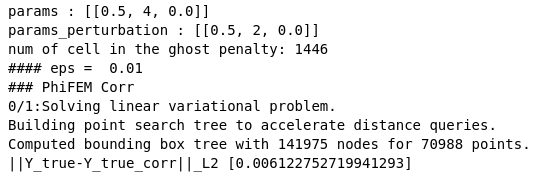
\includegraphics[width=0.5\linewidth]{test_kernel.png}
\end{minipage}

\subsection{Résultat Correction $\mathbb{P}^3$ et $\mathbb{P}^5$ (Legendre)}

\begin{minipage}{\linewidth}
	\centering
	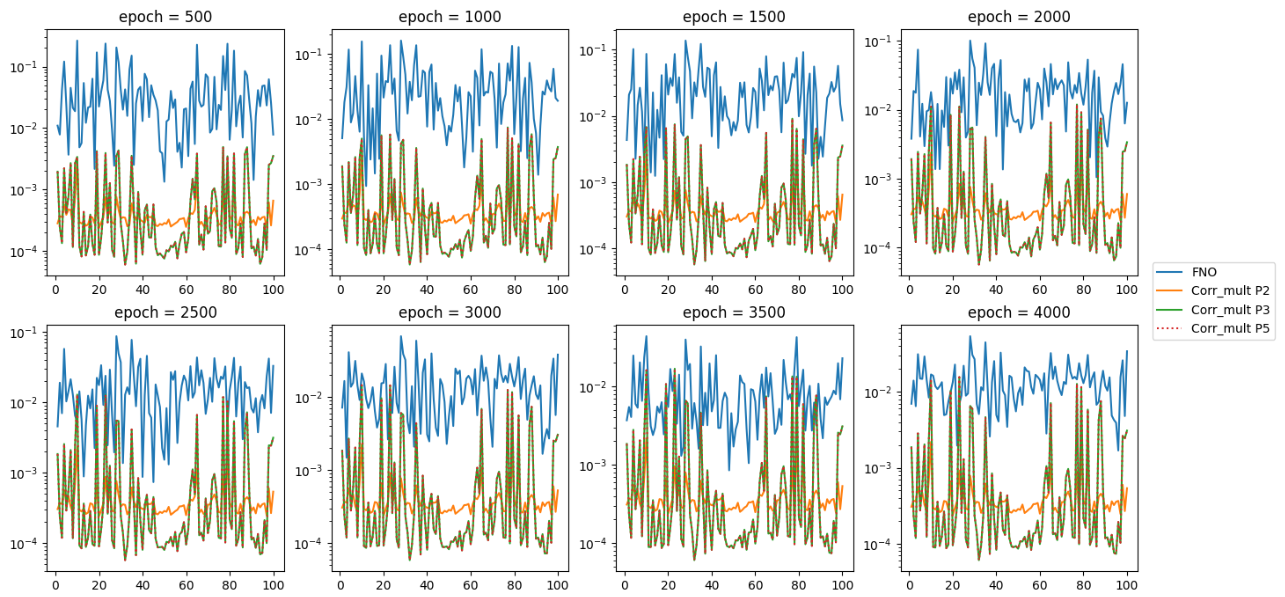
\includegraphics[width=0.8\linewidth]{test_Corr_P3_P5.png}
\end{minipage}

\subsection{Test de convergence 1D (Legendre)}

Test de convergence de la décomposition en une série de polynôme de Legendre sur la solution analytique suivante
$$u_{ex}(x) = \exp\left(-\frac{(x-\mu)^2}{2\sigma^2}\right)$$
avec $\mu=0$ et $\sigma=1$.

On comparera pour différents nombres de points $N$, l'erreur max(|Y\_true-Y\_true\_reconsrtruct|) en faisant varier le nombre de polynômes de Legendre $P$. On a commencé par test en considérant une solution discrétisée en nos $N^2$ nœuds et en utilisant la méthode des trapèzes pour calculer les coefficients $\alpha_p$. Etant donné que les résultats n'étaient pas bons, on a testé avec une une méthode de quadrature de scipy (\href{https://docs.scipy.org/doc/scipy/reference/generated/scipy.integrate.quad.html#scipy.integrate.quad}{scipy.integrate.quad}) qui prend une expression analytique de notre fonction en paramètre.

\begin{Rem}
	On notera que contrairement à la méthode des trapèzes, avec scipy le paramètre $N$ n'influence pas le calcul des coefficients. On calcule juste l'erreur en norme infini sur des solutions avec différents nombres de points.
\end{Rem}

Résultats obtenus avec la méthode des trapèzes :

\begin{minipage}{\linewidth}
	\centering
	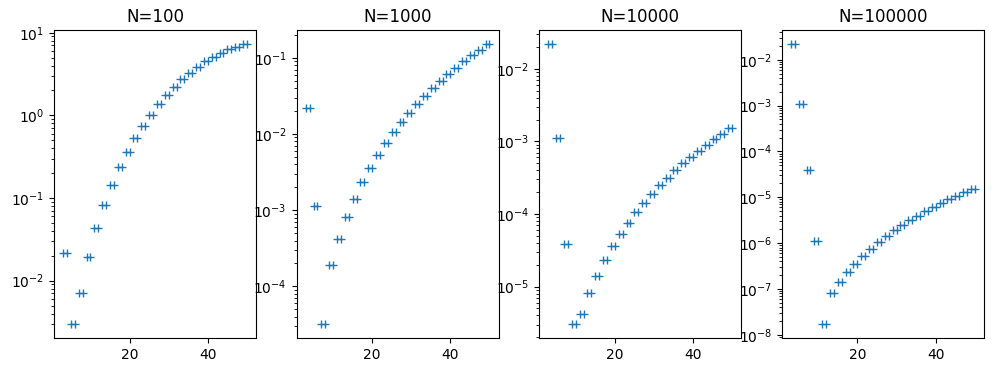
\includegraphics[width=0.65\linewidth]{test_cvg_trapeze.png}
\end{minipage}

Résultats obtenus avec la méthode de scipy :

\begin{minipage}{\linewidth}
	\centering
	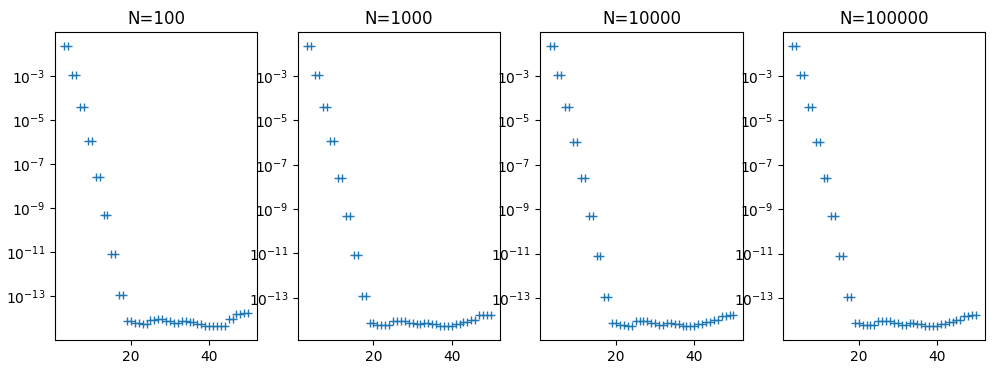
\includegraphics[width=0.65\linewidth]{test_cvg_scipy.png}
\end{minipage}

\subsection{Documentation sphinx}

\begin{minipage}{\linewidth}
	\centering
	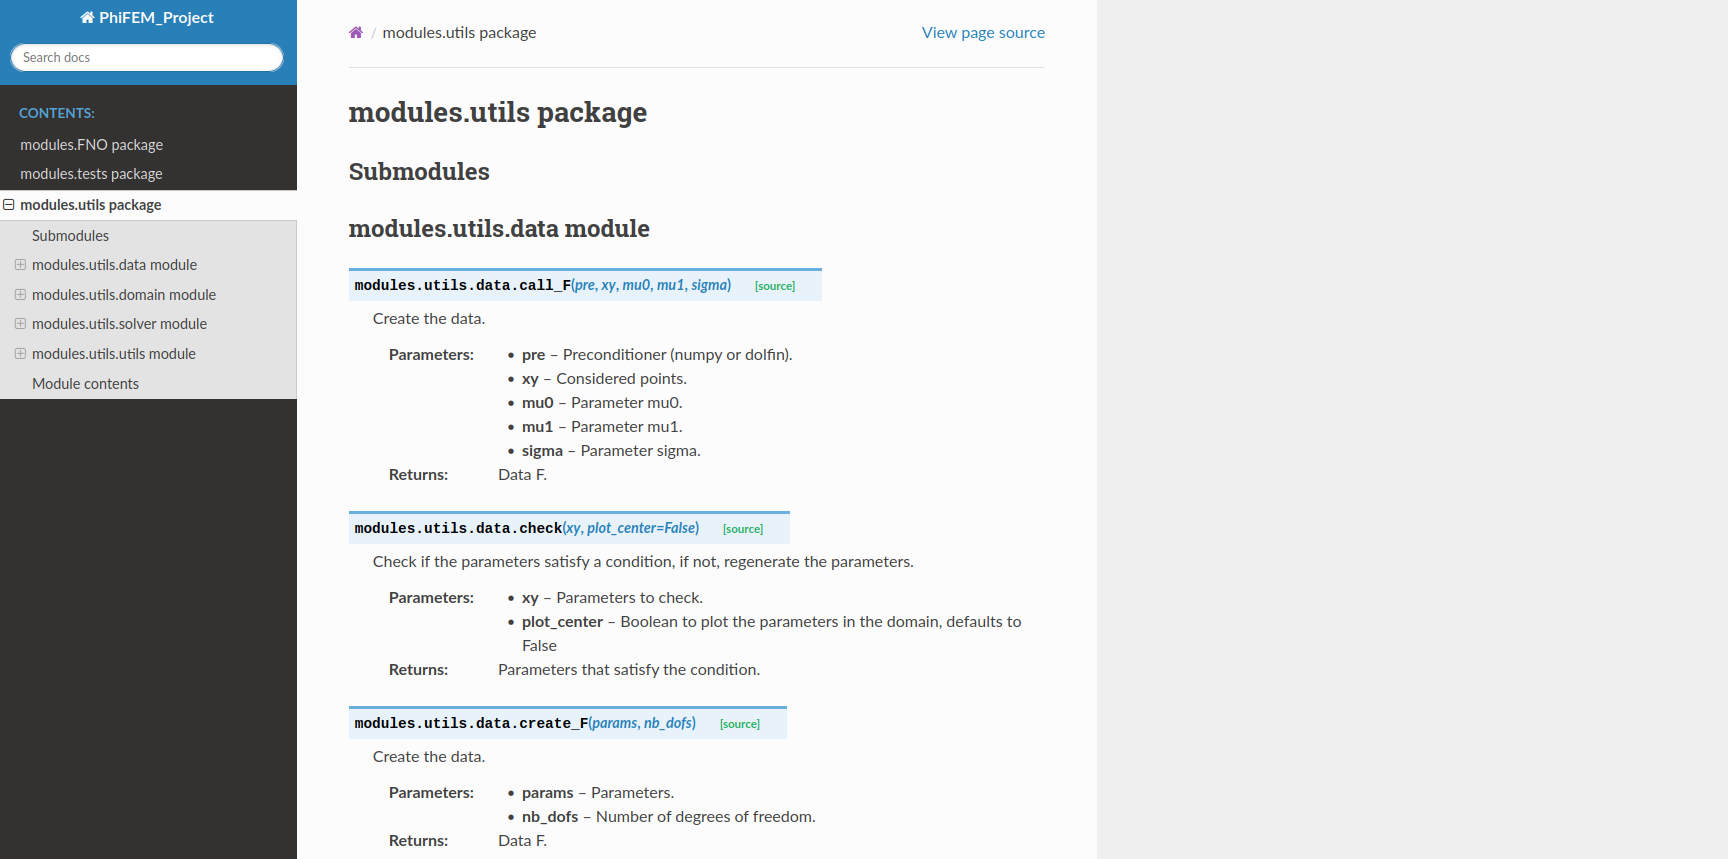
\includegraphics[width=0.7\linewidth]{doc_sphinx.png}
\end{minipage}

\subsection{Estimation d'erreur - Problème rehaussé (Modif !) \faBookmarkO}

On se place ici dans le cadre de FEM standard. 

\textbf{Problème initital :} \\
On considère initialement le problème de Poisson avec condition de Dirichlet homogène ou non homogène :
\begin{equation}
	\left\{\begin{aligned}
		&-\Delta u=f \quad &&\text{dans } \Omega \\
		&u=g \quad &&\text{sur } \Gamma
	\end{aligned}\right. \label{pb_initial} \tag{$\mathcal{P}$}
\end{equation}

\textbf{Problème considéré :} \\
Dans notre cas, on souhaite appliquer une correction à la sortie d'un FNO.
On va considérer ici que l'on possède une solution analytique $u_{ex}$ et qu'après une utilisation du FNO, on obtient une solution du type
$$\tilde{\phi}(x,y) = u_{ex}(x,y)-\epsilon P(x,y)$$
avec $P$ la perturbation (tel que $P=0$ sur $\Gamma$) et $\epsilon$ petit.

On considère
$$\hat{\phi}=\tilde{\phi}+m=u_{ex}-\epsilon P+m=\widehat{u_{ex}}-\epsilon P$$
avec $\widehat{u_{ex}}=u_{ex}+m$ et $m$ une constante.

On souhaite alors résoudre le problème suivant :
\begin{equation}
	\left\{\begin{aligned}
		&-\Delta (\hat{\phi}C)=f \quad &&\Omega \\
		&(\hat{\phi}C)=g+m \quad &&\Gamma
	\end{aligned}\right. \label{pb_reh} \tag{$\mathcal{C}$}
\end{equation}

On pose alors
$$\hat{u}=\hat{\phi}C$$

\textbf{But du document :} \\
Démonter la propriété suivante :
\begin{equation}
	\left|\left|\hat{u}-\hat{u_h}\right|\right|_0\le ch^{k+1}||\hat{\phi}||_\infty\left|C\right|_{k+1}
	\label{ine_a_dem}
\end{equation}

\textbf{Problèmes variationnels :} \\

Problème variationnel :
$$\text{Trouver } \hat{u}\in V \text{ tel que } a(\hat{u},v)=l(v), \;\forall v\in V$$

Problème variationnel approché :
$$\text{Trouver } \hat{u_h}\in V_h \text{ tel que } a(\hat{u_h},v_h)=l(v_h), \;\forall v_h\in V_h$$

\subsubsection*{Partie 1 : norme $H^1$}

Comme $V_h$ est un sous espace vectoriel de $V$, en posant $v=v_h$, on obtient :
$$a(\hat{\phi}C,\hat{\phi}v_h)-a(\hat{\phi}C_h,\hat{\phi}v_h)=0 \quad \forall v_h\in V_h$$
On a alors l'orthogonalité de Galerkin : \color{red}{(ATTENTION : Abus de notation sur $v_h$ !)}\color{black}
$$a(\hat{u}-\hat{u_h},v_h)=0 \quad \forall v_h\in V_h$$
On a alors
\begin{align*}
	\color{red}{\nu}\color{black}||\hat{u}-\hat{u_h}||_1^2&\le\alpha a(\hat{u}-\hat{u_h},\hat{u}-\hat{u_h}) &&\text{par coercivité} \\
	&=\alpha a(\hat{u}-\hat{u_h},\hat{u}-I_h\hat{u}+I_h\hat{u}-\hat{u_h}) \\
	&=\alpha a(\hat{u}-\hat{u_h},\hat{u}-I_h\hat{u}) &&\text{par orthogonalité de Galerkin en prenant } v_h=\hat{u_h}-I_h\hat{u} \\
	&\le\alpha |\hat{u}-\hat{u_h}|_1|\hat{u}-I_h\hat{u}|_1 &&\text{par continuité} \\
	&\le\alpha ||\hat{u}-\hat{u_h}||_1|\hat{u}-I_h\hat{u}|_1
\end{align*}
Ainsi
$$||\hat{u}-\hat{u_h}||_1\le\alpha|\hat{u}-I_h\hat{u}|_1$$
Or 
$$|\hat{u}-I_h\hat{u}|_1=|(C-I_hC)\hat{\phi}|_1$$
En posant $A=C-I_hC$, on a
$$|A\hat{\phi}|_1=||(A\hat{\phi})'||_0=||A'\hat{\phi}+A\hat{\phi}'||_0\le||A'\hat{\phi}||_0+||A\hat{\phi}'||_0$$
Comme
$$||A'\hat{\phi}||_0=\sqrt{\int_\Omega(A'\hat{\phi})^2}\le \max_\Omega \hat{\phi}\sqrt{\int_\Omega(A')^2}=||\hat{\phi}||_\infty|A|_1\le||\hat{\phi}||_\infty||A||_1$$
et
$$||A\hat{\phi}'||_0=\sqrt{\int_\Omega(A\hat{\phi}')^2}\le \max_\Omega \hat{\phi}'\sqrt{\int_\Omega(A)^2}=||\hat{\phi}'||_\infty||A||_0\le \alpha||\hat{\phi}||_\infty||A||_1$$
Ainsi
$$|A\hat{\phi}|_1\le\alpha ||\hat{\phi}||_\infty||A||_1$$
Donc
$$|\hat{u}-I_h\hat{u}|_1=|(C-I_hC)\hat{\phi}|_1\le\alpha ||\hat{\phi}||_\infty||C-I_hC||_1$$

Finalement en utilisant l'inégalité d'interpolation, on obtient
\begin{equation}
	\boxed{||\hat{u}-\hat{u_h}||_1\le\alpha h^k ||\hat{\phi}||_\infty |C|_{k+1}}
	\label{norme_H1}
\end{equation} 

\subsubsection*{Partie 2 : norme $L^2$}

On applique la méthode de dualité d'Aubin-Nitsche. On considère le problème dual : \\
Soit $\hat{z}\in H_0^1(\Omega)$ solution du problème
$$\left\{\begin{aligned}
	&-\Delta\hat{z}=\hat{e_h} \quad &&\text{dans }\Omega \\
	&\hat{z}=0 \quad &&\text{sur } \Gamma
\end{aligned}\right.$$
avec $\hat{e_h}=\hat{u}-\hat{u_h}$.
Alors
$$a(u,v)=-\int_\Omega\Delta u\cdot v=\int_\Omega\nabla u\cdot\nabla v$$
et comme $e_h\in H_0^1(\Omega)$
\begin{equation}
	a(\hat{z},\hat{e_h})=\int_\Omega(-\Delta \hat{z})\cdot \hat{e_h}=\int_\Omega \hat{e_h}^2=||\hat{e_h}||_0^2
	\label{norme_e_h}
\end{equation}
De plus, par les propriétés de régularité : 
\begin{equation}
	\hat{z}\in H^2(\Omega)
	\label{z_H_2}
\end{equation}
et
\begin{equation}
	||\hat{z}||_2\le \alpha||\hat{e_h}||_0 =\alpha||\hat{u}-\hat{u_h}||_0
	\label{prop_reg}
\end{equation}
Ainsi
\begin{align*}
	||\hat{u}-\hat{u_h}||_0^2&=||\hat{e_h}||_0^2 \\
	&=a(\hat{z},\hat{e_h}) &&\text{par \ref{norme_e_h}} \\
	&=a(\hat{z}-I_h\hat{z},\hat{e_h}) &&\text{par orthogonalité de Galerkin} \\
	&\le\alpha|\hat{z}-I_h\hat{z}|_1|\hat{e_h}|_1 &&\text{par continuité} \\
	&\le\alpha h|\hat{z}|_2|\hat{e_h}|_1 &&\text{par \ref{z_H_2} et par inégalité d'interpolation} \\
	&\le\alpha \cdot h|\hat{z}|_2 \cdot h^k||\hat{\phi}||_\infty |C|_{k+1} &&\text{par \ref{norme_H1}} \\
	&\le\alpha h^{k+1}||\hat{u}-\hat{u_h}||_0||\hat{\phi}||_\infty |C|_{k+1} &&\text{par \ref{prop_reg}}
\end{align*}
Finalement
\begin{equation}
	\boxed{||\hat{u}-\hat{u_h}||_0\le\alpha h^{k+1}||\hat{\phi}||_\infty |C|_{k+1}}
\end{equation}

\begin{Rem}
	On notera que
	$$||\hat{u}-\hat{u_h}||_0=||u+m-(u_h+m)||_0=||u-u_h||_0$$
\end{Rem}

\conclusion{Après une réunion mercredi avec Emmanuel et Michel, Emmanuel a proposé de tester les 2 idées suivantes. La première, tenter de corriger en $\mathbb{P}^{10}$ une solution analytique décomposée en série de polynômes de Legendre. La seconde, implémenter un réseau de neurones multi-perceptron avec $||w_\theta(x)\phi(x)-u(x)||_{H^1}$. Ces deux idées seront abordés dans le suivi de la semaine prochaine.}